\section{One big experiment}\label{sec:1}
Let $P = \num{10000}$ and $X = 1$. Since only one experiment is done,
\cref{eq:pi_final} cannot be used to calculate the uncertainty. Because of that
the uncertainty is defined as
\begin{equation}
	\Delta \pi_x = \sqrt{\text{Var}(4[X^2 + Y^2 \leq 1])}
    \label{eq:uncertainty_for_one_x}
\end{equation}
with $\text{Var}(X)$ being the variance of the random variable $X$.
Letting the experiment run results in a value of
\begin{equation}
	\pi_x = \num{3.1 \pm 1.7},
\end{equation}
which is considering the uncertainty of approximately \per{53} close to the real value.\par
%
When doing just one experiment, the distribution of the generated points is 
of interest. For this the histogram of the radii $R = \sqrt{X^2 + Y^2}$
and the squared radii are plotted in \cref{fig:radii_hist,fig:radii_squared_hist}.
For the radii we can see a linear rising distribution with a maximum at $r=1$, after which 
the distribution drops. 
The linear rise is explainable with the following argumentation:\\
The points generated inside the square are distributed uniformly, but since 
the circumference of a circle is proportional to the radius, the point density $n(r)$
also has to be $n(r)\sim  r$. The drop after $r = 1$ occurs because 
a circle with radius $1$ is the biggest that fits inside a $2\times 2$ 
square, so there will be fewer points that can be generated with that radius.\par 
For the $R^2$ distribution a constant distribution up until $r=1$ is visible.
This can be easily calculated. For two random variables $X, Y$ and 
a function $V: X \rightarrow Y$ and given distribution $n(x)$, the distribution of 
$Y$ can be calculated with the delta distribution $\delta(x)$ by 
\[
    p(y) = \int dx\, n(x) \delta(y - V(x)).
\] 
For the variable $\rho = r^2$ we get 
\begin{align*}
    p(\rho) &= \text{const}\cdot\int_0^1 dr\, r\cdot\delta(r^2 - \rho)
     = \text{const}\cdot\int_0^1 dr\, r \cdot \frac{\delta(r - \sqrt\rho)}{2\sqrt\rho}\\
     &= \text{const }
\end{align*}
\textbf{TO BE CONTINUED}


\begin{figure}[h!]
    \centering
    \begin{minipage}{.45\linewidth}
        \centering
        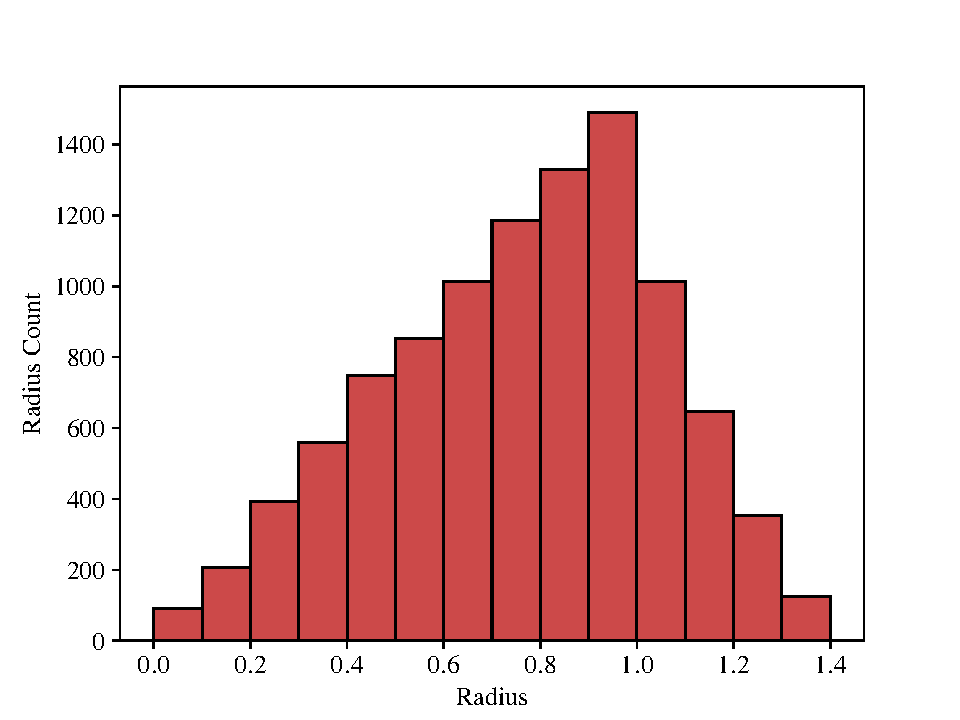
\includegraphics[width=\linewidth]{figs/ex1.1_radii_hist.pdf}
        \caption{Histogram of radii from all the generated points of one big experiment
            with $P=\num{10000}$.}
        \label{fig:radii_hist}
    \end{minipage}
    \hfill
    \begin{minipage}{.45\linewidth}
        \centering
        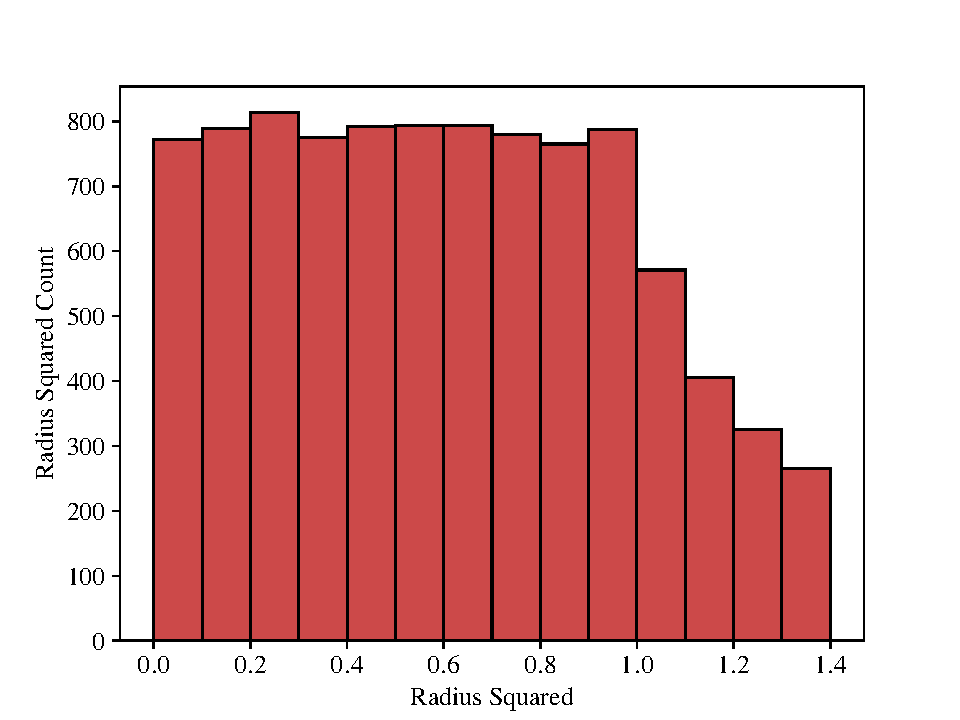
\includegraphics[width=\linewidth]{figs/ex1.1_radii_squared_hist.pdf}
        \caption{Histogram of the squared radii from all the generated points of one big experiment
            with $P=\num{10000}$.}
        \label{fig:radii_squared_hist}
    \end{minipage}

\end{figure}

\begin{figure}[h]
    \centering
    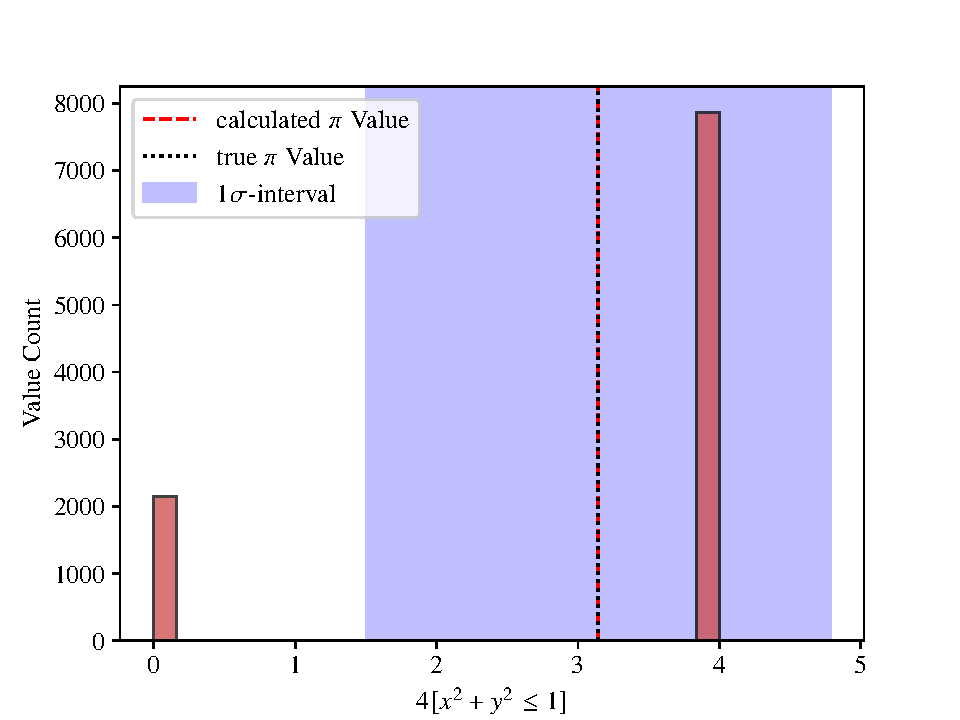
\includegraphics[width=.6\linewidth]{figs/ex1.1_indicator_hist.pdf}
    \caption{Histogram of the indicator variable $[X^2 + Y^2 \leq 1]$ for an experiment 
        with $P = \num{10000}$.}
\end{figure}